\documentclass[conference]{IEEEtran}
\IEEEoverridecommandlockouts
% The preceding line is only needed to identify funding in the first footnote. If that is unneeded, please comment it out.
\usepackage{cite}
\usepackage{amsmath,amssymb,amsfonts}
\usepackage{algorithmic}
\usepackage{graphicx}
\usepackage{textcomp}
\usepackage{xcolor}
\usepackage[ngerman]{babel}
\usepackage[utf8]{inputenc}
\def\BibTeX{{\rm B\kern-.05em{\sc i\kern-.025em b}\kern-.08em
    T\kern-.1667em\lower.7ex\hbox{E}\kern-.125emX}}
 
    
\begin{document}


\title{Implementierung Objektorientierter-Konstrukte in der Java Virtual Machine\\}

\author{\IEEEauthorblockN{Braun Georg}
\IEEEauthorblockA{\textit{Fachhochschule Aachen} \\
Aachen, Deutschland \\
Georg.Braun@alumni.fh-aachen.de}
}

\maketitle

\begin{abstract}

\end{abstract}



\section{Einleitung}
Java ist einer der beliebtesten objektorientierten Programmiersprachen und ist schon seit einigen Jahren eine etabliert. Neben Java gibt es noch diverse andere Programmiersprachen, wie zum Beispiel Kotlin oder Clojure die alle eine elementare Gemeinsamkeit haben. Alle diese Sprachen werden nicht speziell für eine Rechnerarchitektur, sondern in einen Bytecode kompiliert. Dieser Bytecode kann von Java Virtual Machines verarbeitet werden. Somit ist eine Ausführung des Code unabhängig von der zugrunde liegenden Rechnerarchitektur möglich (vorausgesetzt die Java Virtual Machine kann auf dieser betrieben werden). Im Fokus dieses Dokuments steht die Bytecode Repräsentation von objektorientierten Konstrukten. Dazu wird zunächst auf die Struktur der Java Klassen-Dateien eingegangen um darauf die zum Verständnis notwendigen Grundlagen der Struktur der Java Virtual Machine aufzugreifen. Danach findet eine Erklärung statt wie auf Bytecode-Ebene Methoden aufgerufen werden. Neben der Umsetzung von Konstruktor-Aufrufen werden auch die Zugriffe auf Objektfelder und Klassen- bzw. Static-Felder erläutert. Zuletzt wird noch auf die Bytecode-Implementation von Typ-Überprüfungen eingegangen.  

\section{Aufbau der class Datei}
Der Programmcode der Hochsprachen wird beim Kompilieren in Bytecode umgewandelt und für jede verwendete Klasse wird eine entsprechende Klassen-Datei (.class) angelegt. Diese Dateien haben eine klar definierte Struktur die in Tabelle \ref{tab1} aufgelistet ist und auf die im folgenden eingegangen wird. eingegangen wird.


\begin{table}[htbp]
\caption{Reihenfolge und Länge der class-Datei Inhalte}
\begin{center}
\begin{tabular}{|c|c|}
\hline
\textbf{Element} & \textbf{Länge} \\
\hline
Magic & 4 Bytes\\
\hline
Major, Minor Version & 4 Bytes\\
\hline
Constant Pool & variabel \\
\hline
Access Flags & 2 Bytes \\
\hline
This Klasse & 2 Bytes \\
\hline
Basisklasse (super) & 2 Bytes \\
\hline
Interfaces & variabel \\
\hline
Felder & variabel \\
\hline
Methoden & variabel \\
\hline
Attribute & variabel \\
\hline
\end{tabular}
\label{tab1}
\end{center}
\end{table}

%ToDo: Beschreibung der Inhalte der class-Datei. Besser noch konkrete Beispiele dafür mit in die Tabelle aufnehmen
Die Datei startet zunächst mit einem Magic welches vier Byte lang ist und die Datei als eine Java-Klassen-Datei identifiziert. Dieses Magic hat den fixen Wert 0xCAFEBABE. Darauf folgen die Major- und Minor-Versionsinformationen welche die verwendete Compilerversion identifizieren. Die nächsten Bytes beschreiben die Länge des folgenden Constant-Pools. Durch diese Angabe ist der Java Virtual Machine bekannt wie viele der folgenden Bytes zum Constant Pool gehören. Dieser enthält Konstanten die mit der Klasse, beziehungsweise dem Interface assoziiert werden. Der Constant-Pool ist als Array variabler Länge umgesetzt. Auf die Elemente kann später über einen Index-Mechanismus zugegriffen werden. Dabei enthält ein Element zunächst ein Byte welches den Typ spezifiziert. Auf Grundlage dieses Typs werden die darauf folgenden Bytes des Elements interpretiert. Nach dem Constant-Pool werden in zwei Bytes die Access-Flags angegeben. Dabei handelt es sich um Flags die beschreiben ob es sich um eine Klasse oder um ein Interface (\verb|ACC_INTERFACE| Flag) handelt. Zudem werden darüber die Zugriffsrechte bekannt gegeben. Beispielsweise wird für einen public Zugriff das Flag \verb|ACC_PUBLIC| verwendet. In den nächsten zwei Bytes steht die this-Information welche die in dieser Klassen-Datei behandelte Klasse oder Interface definiert. Dazu werden diese zwei Bytes als Index im Constant-Pool interpretiert. Dieser muss an dem gegeben Index ein Element des Typs \verb|CONSTANT_Class| enthalten. Dieser wiederum verweist auf ein String-Element welchen den Namen der Klasse beziehungsweise des Interfaces enthält. Die nächsten zwei Bytes geben die verwendete Elternklasse an. Auch hier werden diese zwei Bytes als Index im Constant-Pool interpretiert. Auch in diesem Element sollte der Typ \verb|CONSTANT_Class| stehen und auf die Elternklasse im String-Format verweisen. Nach dieser Angabe folgen die verwendeten Interfaces. Auch an dieser Stelle geben die ersten zwei Bytes die Anzahl der Interfaces an, sodass die Java Virtual Machine die folgenden Bytes richtig interpretieren kann. Der gleiche Mechanismus (Angabe der Anzahl in den ersten zwei Bytes und darauf folgend der jeweilige Inhalt) wird bei den folgenden Klassen-Datei Inhalten auch verwendet. Das Element Felder enthält eine Beschreibung alle Felder die in der Klasse oder dem Interface deklariert wurden. Geerbte Felder werden hier nicht repräsentiert. Ähnlich verhält es sich bei den folgenden Methoden-Definitionen. Diese enthalten (sofern nicht als abstrakt gekennzeichnet) neben der Deklaration auch die komplette Implementation. Dabei werden neben Instanz-Methoden auch Klassen- und Initialisierungsmethoden angegeben. Als letztes kann die Klassen-Datei noch verschiedene Attribute wie zum Beispiel die verwendete Quell-Datei enthalten. \cite{Venners.1996b} \cite{Lindholm.21.08.2018}

\section{Java Virtual Machine Grundlagen Stack und Heap}

% Quelle: JVM SE Specification!
Die Java Virtual Machine besteht aus verschiedenen Bereichen wobei ich im folgenden besonders den Java Virtual Machine Stack und den Heap hervorheben möchte.

Jeder Thread besitzt einen eigenen Java Virtual Machine Stack der zeitgleich mit der Threaderstellung entsteht. Dieser Stack enthält \verb|Frames|. Bei jedem Methodenaufruf wird ein neues Frame erstellt und auf dem Stack abgelegt. Ein Frame besteht aus einem Operanden-Stack, einem Array von lokalen Variablen und einer Referenz zum Runtime Constant-Pool. Der Operanden-Stack ist ein LIFO-Stack der durch Opcodes manipuliert werden kann. Das Array der lokalen Variablen hat zwei Funktionen. Zunächst enthält es bei einem Methodenaufruf die übergebenen Parameter. Die zweite Funktion ist das Speichern der Werte von lokalen Variablen. Handelt es sich bei einem Methodenaufruf um eine Instanz-Methode, so ist der erste Wert in dem Array (Index 0) eine Referenz auf das beim Aufruf verwendete Objekt (this-Referenz). Beim Runtime Constant Pool handelt es sich um eine Laufzeit-Repräsentation des in den Klassendateien definierten Constant Pools. Dieser Pool wird angelegt sobald eine Klasse oder ein Interface erstellt wird. 

Der Runtime Constant Pool ist wiederum ein Teil der Method Area welche sich im Heap Bereich befindet. Der Heap ist für alle Java Virtual Machine Threads zugänglich und dient als Laufzeitspeicher der von allen Klassen und Interfaces allokiert wird. Die Method Area verwaltet zum Beispiel folgende Informationen der Klassen/Interfaces: Runtime Constant-Pool, Feldinformationen, Methodencode und Konstruktoren. Der (von Objekten) allokierte Speicher im Heap wird dabei nie explizit freigegeben. Diese Aufgabe übernimmt der Garbage Collector. \cite{Lindholm.21.08.2018}



\section{Methodenaufrufe}
\subsection{Ablauf eines Methodenaufrufs}
Sobald eine Methode aufgerufen wird erzeugt die Java Virtual Machine ein neues Frame und legt dieses auf den Frame-Stack. Sofern es sich um eine Instanz-Methode handelt werden im Kontext der aufrufenden Methode und in dessen Frame die Objekt-Referenz und potenzielle Methodenargumente von dem Operanden-Stack genommen und in den Frame der aufgerufenen Methode übergeben (siehe Abbildung \ref{fig:aufrufMethode}). Dort sind die Werte im Array der lokalen Variablen zu finden, wobei die Objekt-Referenz an erster Stelle (Index 0) steht und darauf folgend die potenziellen Methoden-Argumente. 

\begin{figure}[htbp] 
  \centering
     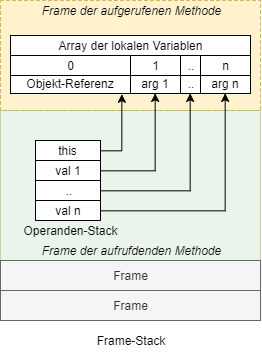
\includegraphics[width=0.4\textwidth]{Grafiken/MethodenAufrufJVM.png}
  \caption{Aufruf einer Instanz-Methode}
  \label{fig:aufrufMethode}
\end{figure}

Falls es sich um den Aufruf einer Klassen-Methode handelt werden nur die Argumente vom Operanden-Stack genommen und das Array der lokalen Variablen in dem Frame der aufgerufenen Methode startet ab Index 0 mit den Methoden-Argumenten. Sobald die Argumente in dem Array vorhanden aktiviert die Java Virtual Machine das neu erzeugte Frame und setzt den Instruktionszeiger auf die erste Instruktion der neuen Methode.\cite{Venners.1997}

\subsection{Vergleich der Methodenaufrufe}
In der Java Virtual Machine kann man zunächst die zuvor angesprochenen zwei Arten von Methoden unterscheiden: Instanz-Methoden und Klassen-Methoden (darunter werden auch die statischen-Methoden) gefasst. Sie unterscheiden sich zunächst darin ob für ihren Aufruf eine Instanz benötigt wird oder nicht. 

Wie bereits zuvor erwähnt können Instanz-Methoden nur in ihrem Instanz-Kontext aufgerufen werden, wobei die aufgerufene Methode von der aktuellen Klasse der Instanz abhängt. Diese Information ist jedoch erst zur Laufzeit des Programms bekannt. Für die Lösung des Problems wird der Mechanismus des late bindings genutzt. Dabei wird beim Aufruf einer Methode der aktuelle Typ des Objekts ermittelt und dieser nach der Methode durchsucht. 

Aufrufe von Klassen-Methoden hingegen basieren auf dem verwendeten Typ einer Referenz welcher sich auch während der Laufzeit nicht ändern. Somit kann bereits während der Komplierung die genutzte Methode bestimmt werden und es ist kein dynamisches Binden notwendig. Hierbei spricht man auch von static (early) binding. Der verwendete Opcode zum Aufruf von Klassen-Methoden ist \verb|invokestatic|. \cite{Venners.1997}

\subsubsection{Dynamic linking}
Die Java Virtual Machine nutzt dynamisches Linken. Einträge in den Runtime Constant Pools welche auf Methoden verweisen sollen sind somit zunächst nur symbolisch (symbolische Referenzen). Ein solche symbolische Referenz ist eine Sammlung von Informationen welche unter anderem den Klassennamen, Methodennamen und Methoden-Deskriptor enthält. Der Methoden-Deskriptor enthält den Rückgabewert der Methode, sowie Anzahl und Typen der Methoden-Argumente). Wird nun eine Methode zur Laufzeit das erste Mal aufgerufen, muss die symbolische Referenz erst aufgelöst werden. Durch die Informationen in der Referenz kann die Java Virtual Machine nach der benötigten Methode suchen und anschließend die symbolische Referenz durch eine direkte Referenz ersetzen. Somit ist für einen weiteren Aufruf der Methode keine erneute Suche notwendig.\cite{Venners.1997}

\subsubsection{Instanz-Methoden}
Neben dem zuvor erwähnten Opcode \verb|invokevirtual| zum Aufruf von Instanz-Methoden gibt es noch zwei weitere Varianten dieses Opcodes welche je nach Kontext verwendet werden. 

Der erste Opcode ist \verb|invokespecial| welcher in Situationen genutzt wird in denen es notwendig ist eine Instanz-Methode basierend auf dem Typ der Referenz (und nicht des Objekts) aufzurufen. In diesem Fall wird auch kein dynamisches Binden benötigt. Eine solche Situation ist zum Beispiel die Instanz-Initialisierung welche über die sogenannten Init-Methoden erfolgt. Diese Init-Methoden enthalten den Konstruktur-Code. Jede Klasse hat für jeden Konstruktur eine Init-Methode (wird kein Konstruktor explizit definiert wird eine Standard Init-Methode angelegt). Sobald eine neue Instanz angelegt wird findet der Aufruf einer der Init-Methode statt. Innerhalb dieser wird entlang der Vererbungshierarchie die Init-Methoden der jeweiligen vererbenden Klassen aufgerufen. Für diesen Aufruf ist die Verwendung von \verb|invokespecial| vorgesehen. Eine ähnliche Situation für die Verwendung des Opcode ist der Aufruf von überschriebenen Instanz-Methoden. Wird die Implementation der vererbenden Klasse mit dem Schlüsselwort \textit{super} aufgerufen, so findet der Aufruf im Bytecode ebenfalls mit \verb|invokespecial| statt.

% ToDo: invokeinterface
Eine weitere Variante ist die Verwendung von \verb|invokeinterface|. Diese wird verwendet wenn die zugrundeliegende Referenz ein Interface ist. Ansonsten ist die Funktionsweise sehr ähnlich zu \verb|invokevirtual|. Wenn die Java Virtual Machine eine Klassen-Datei lädt wird (je nach der verwendeter Java Virtual Machine Implementation) eine Methoden-Tabelle für die Klasse erzeugt. Diese Tabelle enthält die direkten Referenzen zu den Bytecodes der Methoden welche bei einer Instanz dieser Klasse aufgerufen werden können. Die Tabelle beinhaltet dabei auch die Methoden der Oberklassen. Findet ein Methoden-Aufruf auf Basis einer Klassen-Referenz statt ist die Reihenfolge der Methodendefinitionen fix, sodass die Java Virtual Machine sich sicher sein an welcher Stelle (Offset) in der Tabelle die benötigte Methode steht. Die gleiche Methode kann aber gegebenenfalls auch über unterschiedliche Interfaces angesprochen werden wobei nicht unbedingt klar ist an welcher Position in der Methoden-Tabelle die Methode zu finden ist. Deshalb muss die Methode bei jedem Aufruf über ein Interface neu gesucht werden was wiederum einen gesonderten Aufruf mit dem Opcode \verb|invokeinterface| notwendig macht.\cite{Venners.1997}

\subsection{Beispielprogramm}

\section{Konstruktor}

\section{Zugriff auf Felder}
\subsection{Zugriff auf Objekt-Felder}
\subsection{Zugriff auf Klassen-/Static-Felder}

\section{Typüberprüfung}

\bibliographystyle{ieeetr}
\bibliography{literatur} 

\end{document}
